\documentclass[a4paper]{article}
\usepackage[utf8]{inputenc}
\usepackage[spanish, es-tabla, es-noshorthands]{babel}
\usepackage[table,xcdraw]{xcolor}
\usepackage[a4paper, footnotesep=1.25cm, headheight=1.25cm, top=2.54cm, left=2.54cm, bottom=2.54cm, right=2.54cm]{geometry}
%\geometry{showframe}

%\usepackage{wrapfig}			%Wrap figure in text
\usepackage[export]{adjustbox}	%Move images
\usepackage{changepage}			%Move tables

\usepackage{tikz}
\usepackage{amsmath}
\usepackage{amsfonts}
\usepackage{amssymb}
\usepackage{float}
\usepackage{graphicx}
\usepackage{caption}
\usepackage{subcaption}
\usepackage{multicol}
\usepackage{multirow}
\usepackage{wrapfig}
\setlength{\doublerulesep}{\arrayrulewidth}
\usepackage{booktabs}
\usepackage[numbib, nottoc, notlot, notlof]{tocbibind}

\usepackage{hyperref}
\hypersetup{
    colorlinks=true,
    linkcolor=blue,
    filecolor=magenta,      
    urlcolor=blue,
    citecolor=blue,    
}

%Change Font Size

% #1 = size, #2 = text
\newcommand{\setparagraphsize}[2]{{\fontsize{#1}{6}\selectfont#2 \par}}		%Cambia el size de todo el parrafo
\newcommand{\setlinesize}[2]{{\fontsize{#1}{6}\selectfont#2}}				%Cambia el font de una oración

\newcommand{\note}[1]{
	\begin{center}
		\huge{ \textcolor{red}{#1} }
	\end{center}
}

%FONTS (IMPORTANTE): Compilar en XeLaTex o LuaLaTeX
\usepackage{anyfontsize}	%Font size
\usepackage{fontspec}		%Font type

\usepackage{etoolbox}
\usepackage{todonotes}

\newcommand{\observacion}[2]{  \ifnumequal{1}{#1}{ { \todo[inline,backgroundcolor=red!25,bordercolor=red!100]{\textbf{Observación: #2}} } }{  }  }

\setcounter{topnumber}{2}
\setcounter{bottomnumber}{2}
\setcounter{totalnumber}{4}
\renewcommand{\topfraction}{0.85}
\renewcommand{\bottomfraction}{0.85}
\renewcommand{\textfraction}{0.15}
\renewcommand{\floatpagefraction}{0.8}
\renewcommand{\textfraction}{0.1}
\setlength{\floatsep}{5pt plus 2pt minus 2pt}
\setlength{\textfloatsep}{5pt plus 2pt minus 2pt}
\setlength{\intextsep}{5pt plus 2pt minus 2pt}

\newcommand{\quotes}[1]{``#1''}
\usepackage{array}
\newcolumntype{C}[1]{>{\centering\let\newline\\\arraybackslash\hspace{0pt}}m{#1}}
\usepackage[american]{circuitikz}
\usetikzlibrary{calc}
\usepackage{fancyhdr}
\usepackage{units} 

\graphicspath{{../Control de posición no lineal/}{../Control de fuerza no lineal/}{../Control híbrido no lineal/}{../Referencias/}{../Deducción de modelo/}{../Conclusiones/}}

\pagestyle{fancy}
\fancyhf{}
\lhead{22.99 - Automación Industrial}
\rhead{Lambertucci, Londero B., Maselli, Mechoulam}
\rfoot{Página \thepage}

%Items con bullets y no cuadrados
\renewcommand{\labelitemi}{\textbullet }


\begin{document}

%%%%%%%%%%%%%%%%%%%%%%%%%
%		Caratula		%
%%%%%%%%%%%%%%%%%%%%%%%%%

\begin{titlepage}
\newcommand{\HRule}{\rule{\linewidth}{0.5mm}}
\center
\mbox{\textsc{\LARGE \bfseries {Instituto Tecnológico de Buenos Aires}}}\\[1.5cm]
\textsc{\Large 22.90  Automaci\'on Industrial}\\[0.5cm]


\HRule \\[0.6cm]
{ \Huge \bfseries Segundo Parcial}\\[0.4cm] 
\HRule \\[1.5cm]


{\large

\emph{Alumno:}\\
\vspace{3pt}

\begin{tabular}{lr} 	
\textsc{Lambertucci}, Guido Enrique  & 58009 \\

\end{tabular}

\vspace{20pt}

\emph{Profesores}\\
\textsc{Arias}, Rodolfo Enrique  \\
\vspace{3pt}
\textsc{Spinelli}, Mariano Tomás \\	
\vspace{3pt}
\textsc{Avogadro}, Federico Sofio \\	
\vspace{3pt}
\vspace{100pt}

\begin{tabular}{ll}

Presentado: & 18/11/21\\

\end{tabular}

}

\vfill

\end{titlepage}

%%%%%%%%%%%%%%%%%%%%%
%		Indice		%
%%%%%%%%%%%%%%%%%%%%%

\tableofcontents
\newpage

%%%%%%%%%%%%%%%%%%%%%
%		Informe		%
%%%%%%%%%%%%%%%%%%%%%

\section{Simulación del Carro con Péndulo Simple}

Para la simulación del carro con péndulo simple se creó un modelo de este utilizando Simscape de Simulink, utilizando una máscara para poder modificar posteriormente los siguientes parámetros:

\begin{itemize}
\item Masa del carro
\item Masa del péndulo
\item Longitud del Péndulo
\end{itemize}

\begin{figure}[H]
	\centering
	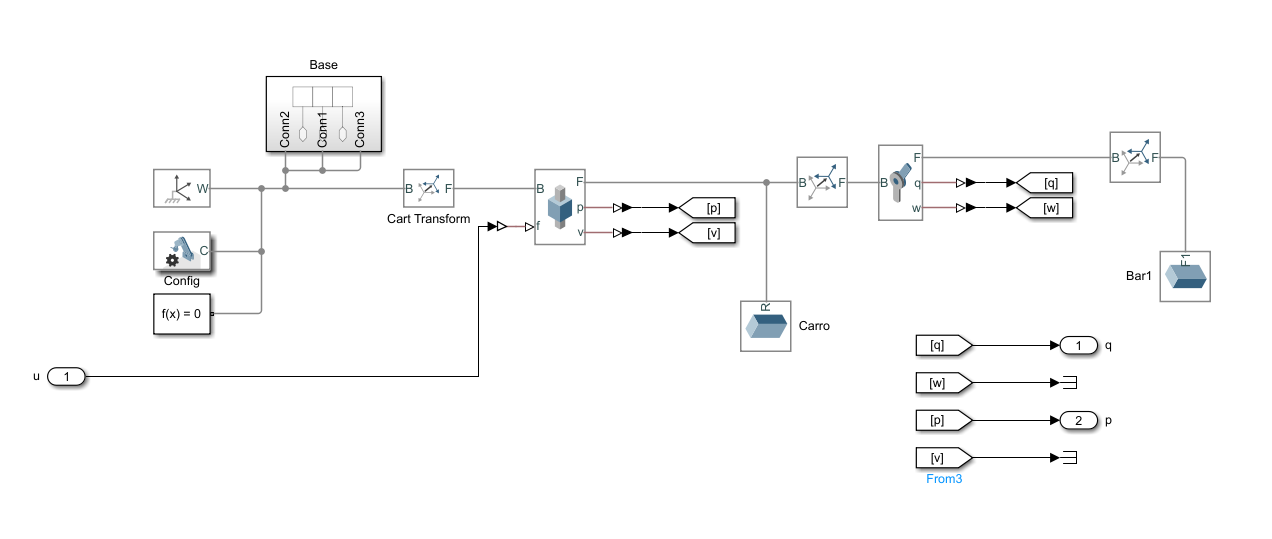
\includegraphics[width=1\linewidth]{Imagenes/Simscape}
	\caption{Modelo de Simscape utilizado como planta.}
	\label{1_simscape}
\end{figure}


\section{Carro con Péndulo Simple: Control en Cascada por Loop Shaping}

Para el control del sistema por loop shaping, como primer paso, se asignaron las variables del modelo de la siguiente forma:

\begin{itemize}
\item Masa del carro = $1 \ kg$
\item Masa del péndulo = $0.25 \ kg$
\item Longitud del Péndulo = $8 \ m$
\end{itemize}

Luego, se utilizó el Model Linearizer de Simulink para linealizar la planta alrededor de $q=0$, $p=0$ y $f=0$; siendo $q$ el ángulo del péndulo, $p$ la posición del carrito y $f$ la fuerza aplicada al carrito.

\begin{figure}[H]
	\centering
	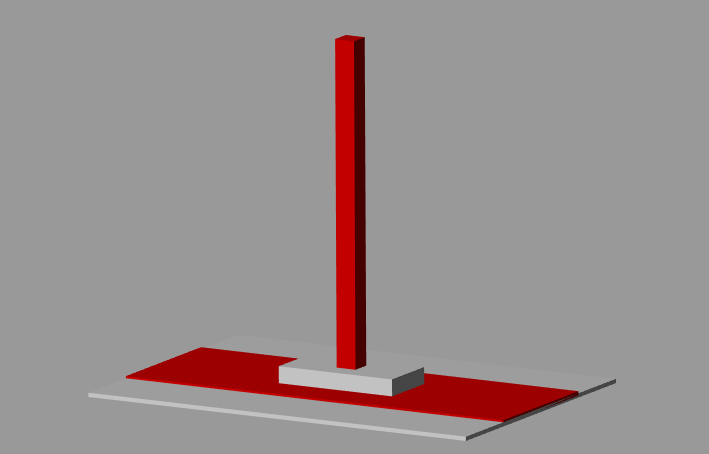
\includegraphics[width=0.5\linewidth]{Imagenes/equilibrio}
	\caption{Punto de equilibrio de linealización.}
	\label{1_equilibrio}
\end{figure}

De esta manera, se obtuvo la siguiente transferencia desde la fuerza aplicada al carrito al ángulo del péndulo:

\begin{equation}
\frac{Q(s)}{F(s)} = \frac{0.1763}{(s-1.47)(s+1.47)}
\end{equation}

donde se nota la presencia de un polo en el semiplano derecho.

Se cierra un lazo de realimentación, tomando el valor de $q$ e inyectándolo a la entrada con una ganancia de valor $-1$ y se grafica la respuesta en frecuencia del sistema viendo solamente el ángulo $q$, obteniendo:

\begin{figure}[H]
	\centering
	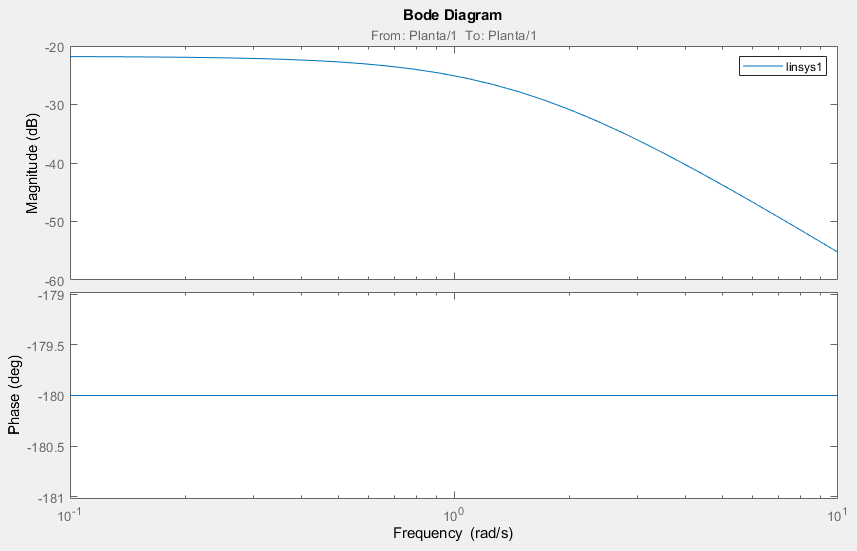
\includegraphics[width=0.8\linewidth]{Imagenes/bode_cerrando_q}
	\caption{Respuesta en frencuencia del sistema entre la fuerza aplicada al carrito y el ángulo del péndulo.}
	\label{bode_cerrando_q}
\end{figure}

donde se observa, como se esperaba, que el sistema es inestable. Notando el polo en el semiplano derecho en $1.47 \frac{rad}{s}$, se decide utilizar un controlador que agregue adelanto de fase para obtener una frecuencia de cruce en $w_{cruce} > 1.7 * w_{rhp} = 2.5 \frac{rad}{s}$, eligiendo entonces agregar un cero de $10 \frac{rad}{s}$, quedando entonces:

\begin{equation}
C_2(s) = \frac{s-10}{s-100}
\end{equation} 

Cabe notar que se agregó un polo rápido que no afecte la dinámica del sistema en $100 \frac{rad}{s}$ para lograr un controlador propio.

Luego, se graficó nuevamente la respuesta en frecuencia, obteniendo:

\begin{figure}[H]
	\centering
	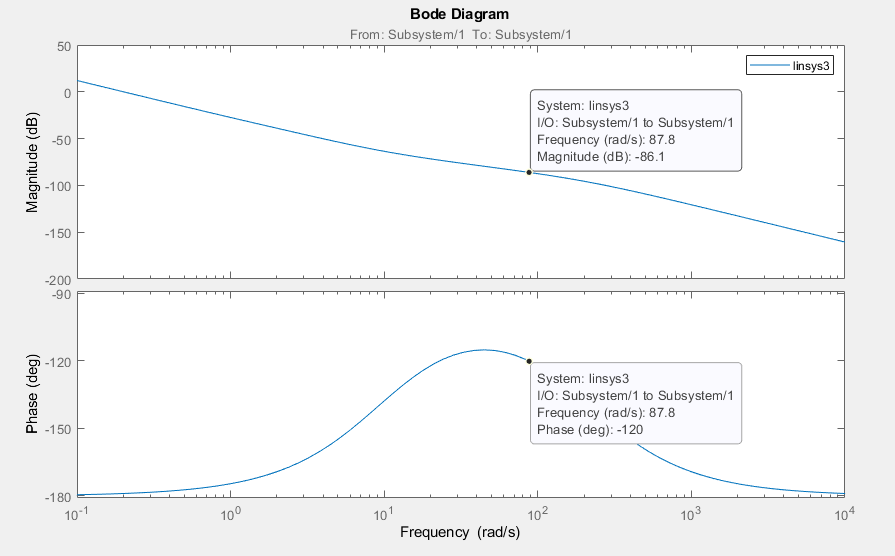
\includegraphics[width=0.8\linewidth]{Imagenes/bode_cerrando_q_con_controlador}
	\caption{Respuesta en frencuencia del sistema entre la fuerza aplicada al carrito y el ángulo del péndulo con controlador.}
	\label{bode_cerrando_q_con_controlador}
\end{figure}

Se busca un margen de fase de $60$ grados, por lo que se agrega una ganancia de $86 dB$ al controlador, calculado como se observa en la Figura (\ref{bode_cerrando_q_con_controlador}). Finalmente, se tiene que

\begin{equation}
C_2(s) = 1.9953e+04 \cdot \frac{s-10}{s-100}
\end{equation}

Se valida el control graficando una última vez la respuesta en frencuencia quedando:

\begin{figure}[H]
	\centering
	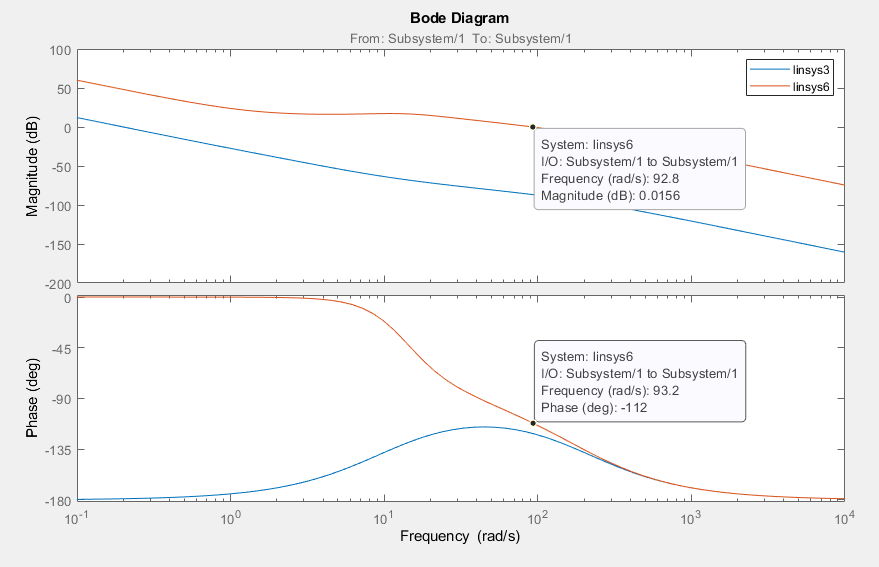
\includegraphics[width=0.8\linewidth]{Imagenes/bode_cerrando_q_con_controlador_ganancia}
	\caption{Respuesta en frencuencia del sistema entre la fuerza aplicada al carrito y el ángulo del péndulo con controlador y frecuencia de cruce ajustada.}
	\label{bode_cerrando_q_con_controlador_ganancia}
\end{figure}

donde se observa que el margen de fase es de $\approx 68$ grados.

En este punto del diseño, si se simula el carrito con un disturbio de ruido blanco de un segundo de frecuencia de muestreo, se puede observar que el ángulo es correctamente estabilizado, sin embargo el carrito presenta drift al no ser controlada la posición de este.

\begin{figure}[H]
	\centering
	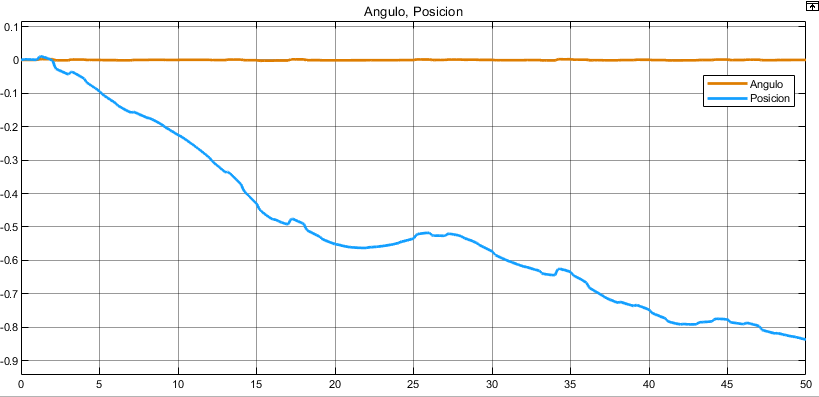
\includegraphics[width=0.8\linewidth]{Imagenes/simulacion_solo_angulo}
	\caption{Simulación de la planta controlando únicamente el ángulo del péndulo.}
	\label{simulacion_solo_angulo}
\end{figure}

A continuación, se cierra otro lazo de realimentación por afuera del anterior utilizando la posición del carrito y se grafica la respuesta en frecuencia entre la fuerza aplicada al carrito y la posición de este, obteniendo el siguiente resultado:

\begin{figure}[H]
	\centering
	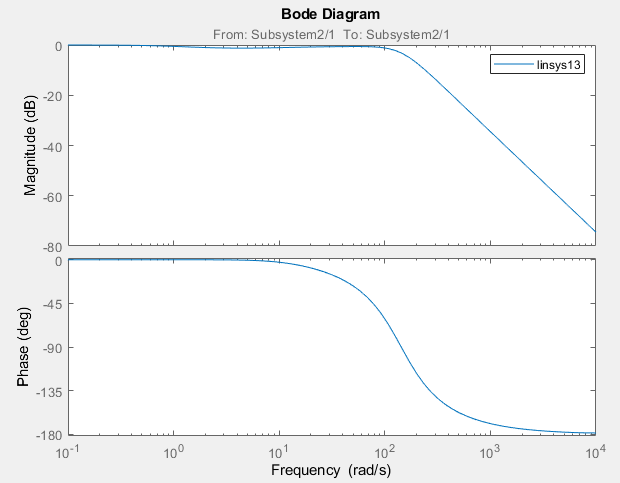
\includegraphics[width=0.8\linewidth]{Imagenes/bode_cerrando_p}
	\caption{Respuesta en frecuencia entre la fuerza aplicada al carrito y la posición de este, cerrando el lazo con realimentación unitaria.}
	\label{bode_cerrando_p}
\end{figure}


\begin{figure}[H]
	\centering
	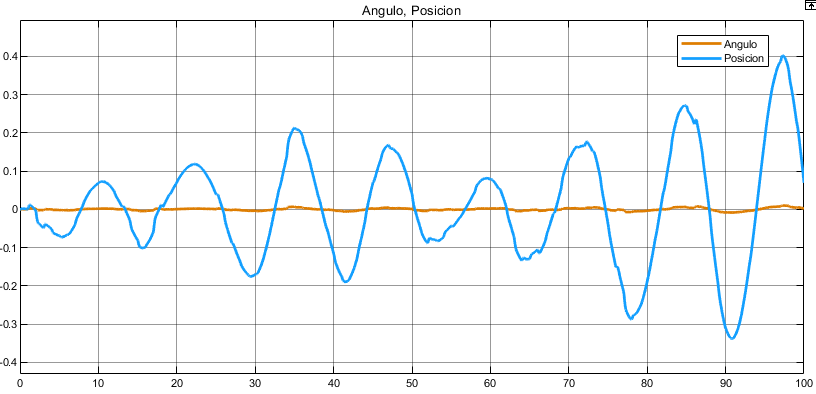
\includegraphics[width=0.8\linewidth]{Imagenes/simulacion_final}
	\caption{Simulación final de la planta controlando el ángulo del péndulo y la posición del carrito.}
	\label{simulacion_solo_angulo}
\end{figure}
\section{Carro con Péndulo Simple: Control por realimentaci\'on de estados.}
 Para la realimentación de estados se tomaron al igual que en loop shaping las matrices producto de la linealizacion de la planta. Se probo que esta sea controlable y observable teniendo como salida el \'angulo y posici\'on del carrito, se observo que no era observable el sistema teniendo únicamente como salida el angulo del carrito, por lo que se opto por conocer tanto la posici\'on como el \'angulo. Y finalmente se realizo una realimetnaci\'on de estados colocando los polos del sistema doble en -3 y doble en -2. Ademas se diseño un observador de estados  para el sistema que permita realizar la realimentación de estados mirando la salida. Tambien se discretizo el observador, y se hizo un control por realimentaci\'on de estados con observador discreto.
\end{document}
